\documentclass{article}
\usepackage{graphicx} % Required for inserting images
\usepackage{biblatex}
\usepackage{float}


\bibliography{report}
\begin{document}

\title{\textbf{CS104 PROJECT REPORT} : \\Python Web Crawler}
\author{Vishal Bysani \\22B1061}
\date{14 June 2023}
\maketitle


\section*{Introduction}
I am Vishal Bysani. I have made a web crawler using Python for the CS104 project. \\
A web crawler, crawler or web spider, is a computer program that's used to search and automatically index website content and other information over the internet. These programs, or bots, are most commonly used to create entries for a search engine index.
\section*{Libraries}
The libraries and dependencies used in this project are:
\begin{itemize}
\item \textbf{argparse} : This library helps in parsing the command line arguments\cite{3}
\item \textbf{BeautifulSoup} : Beautiful Soup is a Python library for getting data out of HTML, XML, and other markup languages. 
\item \textbf{requests} : Python requests is a library for making HTTP requests. It provides an easy-to-use interface that makes working with HTTP very simple, which means it simplifies the process of sending and receiving data from websites by providing a uniform interface for both GET and POST methods.
\item \textbf{Numpy and Matplotlib} : I used matplotlib to generate the plots of the files distribution at various levels recursed by the web crawler\cite{1}
\item \textbf{warnings} : I used this library to not display unnecessary warnings.
\end{itemize}
\section*{Usage}
The web crawler is run using the command:\\
\texttt{python3 Web\_Crawler.py -u <site-name> -t <threshold> -o <output-filename> -s <user-input>}

\begin{itemize}
    \item -u: for the URL. This is a compulsory argument and must print an error if not provided
    \item -t: for the threshold of recursiveness. It must be greater than zero. If not provided, the web crawler will recurse till the end. In case of invalid ( negative values ), it must print an error
    \item -o: For an output file. If not provided then by default print on the command line.
    \item -s: If the user gives 'Y' argument, then the web crawler computes and prints the files sizes as well. It only prints the links if anything else is given as argument.
\end{itemize}
\section*{Code Structure}
\subsection*{Function of base code}
Using the base code from \cite{2}, we can scrape all urls from the given site and prints them all. However, it doesn't crawl into these urls again. Figure \ref{fig:Design1} was taken from \cite{2}
\begin{figure}[H]
    \centering
    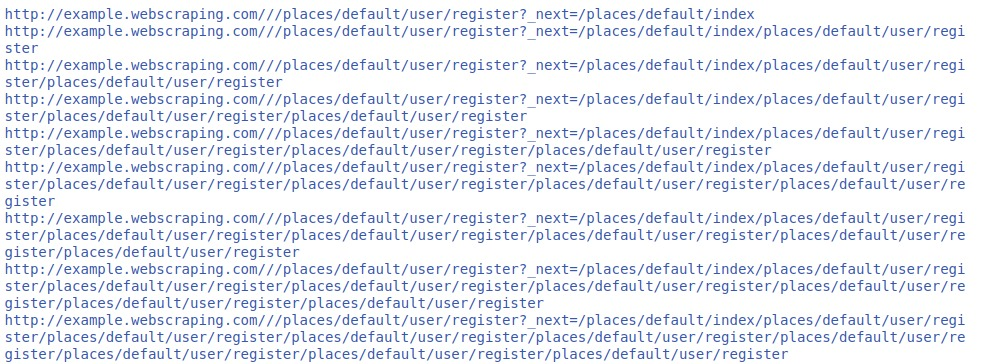
\includegraphics[scale=0.4]{Screenshot.jpeg}
    \caption{Output of a basic Web crawler}
    \label{fig:Design1}
\end{figure}
\subsection*{Implementation of modified code}
I have modified the code from \cite{2} in the following manner to meet the requirements of the problem statement:
\begin{itemize}
    
    \item The code first extracts all the links in the \textit{href} and \textit{src} tags using BeautifulSoup and then modifies them to make valid urls. 
    \item The code recursively crawls through the url provided by the use upto a specified threshold or until the end if not specified.
    \item  The code also segregates all the files at a particular recursion level into various categories like HTML, CSS, JS, JPG, PNG and Others.
\end{itemize}

\subsection*{Customization}
\begin{itemize}
    \item The code keeps printing the number of files and the url crawled by it to indicate the progress of the program.\ref{fig:Design4}
    \begin{figure}[H]
    \centering
    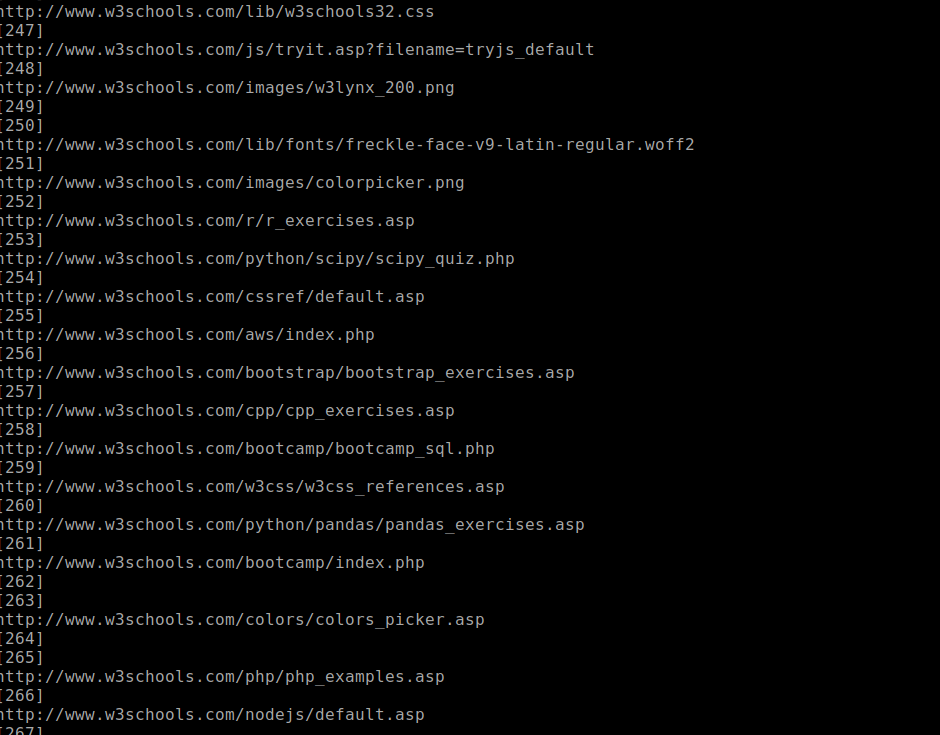
\includegraphics[scale=0.3]{RunningOfTheProgram.png}
    \caption{Indication of running of the program}
    \label{fig:Design4}
\end{figure}
    \item The modified code also identifies if a link is of internal or external domain, and selectively crawls only the internal ones. It separately counts the number of internal and external domain files at each level and prints them in the end.
    \item It also plots bar graphs showing the various categories of files in internal and external domains at each recursion level and saves this plot in Files\_Distribution.png.
    \begin{figure}[H]
    \centering
    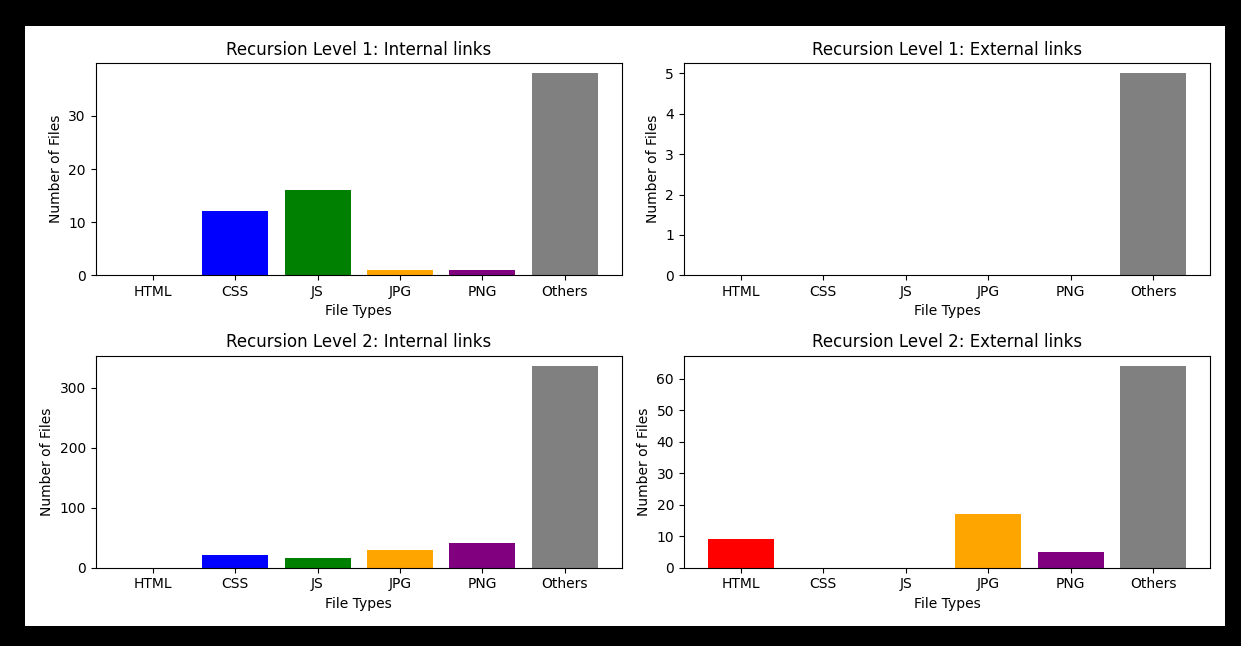
\includegraphics[scale=0.3]{BarGraphs.png}
    \caption{Bar Graph obtained from modified code}
    \label{fig:Design2}
\end{figure}
    \item The code also finds file sizes based upon the argument given by the user to the \texttt{s} tag. 
\end{itemize}


 

\begin{figure}[H]
    \centering
    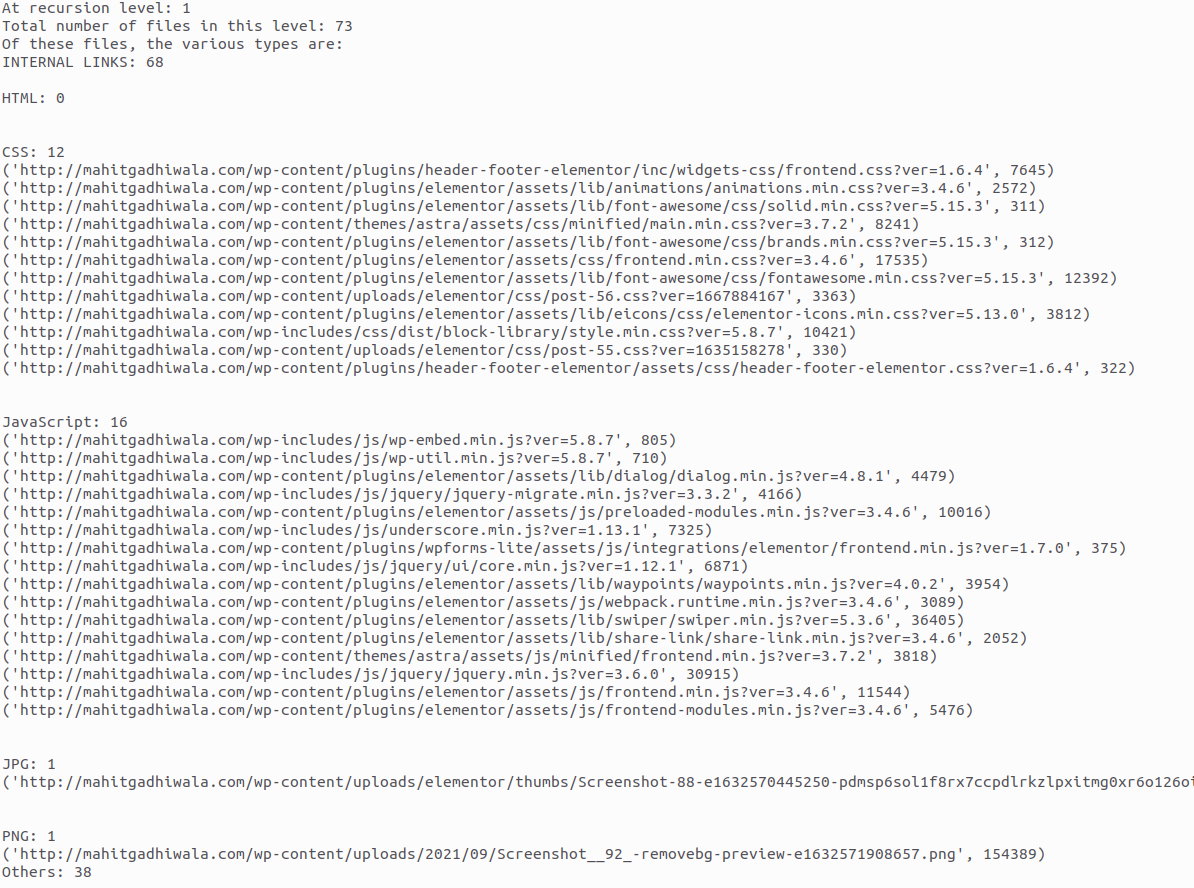
\includegraphics[scale=0.3]{OutputFilePrintFormat.png}
    \caption{Output redirected to the output file}
    \label{fig:Design3}
\end{figure}
As it can be seen from figures \ref{fig:Design2} and \ref{fig:Design3}, the modified web crawler categorizes the files at various recursion levels. Further the web-crawler also finds the file sizes of all the files and prints it along with the links.


\section*{Description of the Submitted Folder}
I have submitted all the files and sub-folder under the folder named \texttt{22B1061\_project}. It includes the following:
\begin{itemize}
\item{Web\_Crawler.py}: It contains the python code.
\item{report.pdf}: It contains the report in the pdf format.
\item{report.tex}: It contains the latex code for the pdf.
\item{report.bib}: It contains all the references I used for this project
\item{BarGraphs.png}: It shows the bar graphs it prints for various recursion levels.
\item{OutputFilePrintFormat.png}: It shows the format in which it prints into the output file given by the user
\item{Screenshot.jpeg}: It shows the output of code which I took as a base for my web crawler.
\end{itemize}
%to print the bibliography

\printbibliography

\end{document}

